\documentclass[10pt]{exam}
\usepackage[phy]{template-for-exam}
\usepackage{pgfplots}
\pgfplotsset{compat=1.18}

\title{Waves \#1}
\author{Rohrbach}
\date{\today}

\begin{document}
\maketitle

\begin{questions}

\question
  The wave below is traveling at 15~m/s.  All measurements are in meters.

  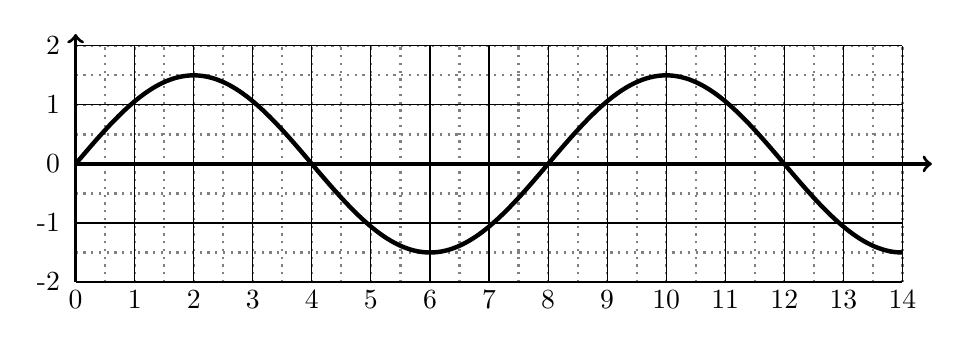
\begin{tikzpicture}[scale=0.75]
    \def\ymax{2}
    \def\xmax{14}
    \draw[dotted,thick,gray] 
      (0,-\ymax*1cm) grid[step=0.5cm] (\xmax*1cm,\ymax*1cm);
    \draw 
      (0,-\ymax*1cm) grid[step=1cm] (\xmax*1cm,\ymax*1cm);
    \foreach \x in {0,...,\xmax}{
      \draw (\x*1cm,-\ymax*1cm) ++(0,-.3cm) node {\x};
    }
    \foreach \y in {-\ymax,...,\ymax}{
      \node[anchor=east] at (-0.1cm,\y*1cm) {\y};
    }
    \draw[very thick,->] 
      (0,0) -- (\xmax*1cm,0) -- ++(0.5cm,0);
    \draw[very thick,->] 
      (0,-\ymax*1cm) -- (0,\ymax*1cm) -- ++(0,0.2cm);

    \draw[ultra thick] (0,0) 
      sin (2, 1.5) cos (4, 0) 
      sin (6,-1.5) cos (8, 0)
      sin (10,1.5) cos (12, 0)
      sin (14,-1.5);
  \end{tikzpicture}

  \begin{parts}
    \part 
      What is the amplitude? \vs
    \part 
      What is the wavelength? \vs
    \part 
      What is the frequency? \vs

  \end{parts}

  
\question
  A buoy on the ocean stays at a stationary location.  An ocean wave comes toward it.  The distance between one crest and the next crest is 6.0~m.  The buoy moves up and down with a frequency of 0.25~Hz.  The amplitude of the wave is 1.0~m.

  \begin{parts}
    \part 
      Draw a picture of this situation.

      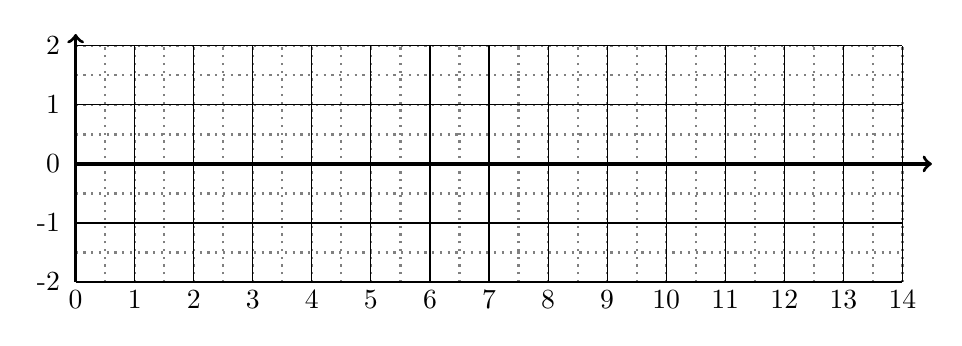
\begin{tikzpicture}[scale=0.75]
        \def\ymax{2}
        \def\xmax{14}
        \draw[dotted,thick,gray] 
          (0,-\ymax*1cm) grid[step=0.5cm] (\xmax*1cm,\ymax*1cm);
        \draw 
          (0,-\ymax*1cm) grid[step=1cm] (\xmax*1cm,\ymax*1cm);
        \foreach \x in {0,...,\xmax}{
          \draw (\x*1cm,-\ymax*1cm) ++(0,-.3cm) node {\x};
        }
        \foreach \y in {-\ymax,...,\ymax}{
          \node[anchor=east] at (-0.1cm,\y*1cm) {\y};
        }
        \draw[very thick,->] 
          (0,0) -- (\xmax*1cm,0) -- ++(0.5cm,0);
        \draw[very thick,->] 
          (0,-\ymax*1cm) -- (0,\ymax*1cm) -- ++(0,0.2cm);
    
        %\draw[ultra thick] (0,1) 
        %  cos (1.5, 0) sin (3, -1) 
        %  cos (4.5, 0) sin (6, 1)
        %  cos (7.5, 0) sin (9, -1)
        %  cos (10.5,0) sin (12,1);
      \end{tikzpicture}

    \part 
      What is the wavelength of the wave?  \vs
    \part 
      What is the period of the wave? \vs
    \part
      How fast is the wave travelling? \vs

  \end{parts}
  

\pagebreak


\question
  If a child on a swing goes back and forth (one oscillation) 11 times in 30 seconds, find her period and frequency. \vs 

\question
  Why does it make sense that a wave with a higher frequency also must have a shorter wavelength?
  \vs


\question
  A sound wave has a wavelength of 2.13 m and a frequency of 160 Hz, what is the velocity of the wave?
  \vs

\question
  The radio station WZPL broadcasts at a frequency of \SI{99.5}{\mega\hertz} (that's \SI{99.5e6}{\hertz}).  Radio waves travel at a speed of \SI{3.00e8}{\meter\per\second}.  How long is the wavelength of WZPL's radio waves?
  \vs

\end{questions}

\end{document}